\documentclass[12pt,a4paper]{article}

% ── Packages ──────────────────────────────────────────────────────────────────
\usepackage[margin=2.5cm]{geometry}
\usepackage{amsmath, amssymb, amsthm}
\usepackage{mathtools}
\usepackage{tikz}
\usetikzlibrary{arrows.meta, positioning, decorations.pathreplacing, calc, shapes.geometric}
\usepackage{pgfplots}
\pgfplotsset{compat=1.18}
\usepgfplotslibrary{polar}
\usepackage{booktabs}
\usepackage{array}
\usepackage[hidelinks]{hyperref}
\usepackage{xcolor}
\usepackage{enumitem}
\usepackage{tcolorbox}
\tcbuselibrary{theorems, skins, breakable}
\usepackage{multicol}
\usepackage{fancyhdr}
\usepackage{lastpage}


% ── Page style ────────────────────────────────────────────────────────────────
\pagestyle{fancy}
\fancyhf{}
\rhead{\small\textit{Further Pure Mathematics 1}}
\lhead{\small\textit{Rayyan Hanif AL25.1}}
\cfoot{\small Page \thepage\ of \pageref{LastPage}}
\renewcommand{\headrulewidth}{0.4pt}

% ── Colour palette ────────────────────────────────────────────────────────────
\definecolor{resultblue}{RGB}{20,80,160}
\definecolor{examplegreen}{RGB}{20,120,60}
\definecolor{basiccol}{RGB}{34,139,34}
\definecolor{medcol}{RGB}{204,102,0}
\definecolor{hardcol}{RGB}{180,0,0}
\definecolor{explorecol}{RGB}{70,50,160}
\definecolor{chaptercol}{RGB}{20,80,160}

% ── tcolorbox environments ────────────────────────────────────────────────────
\newtcbtheorem[number within=section]{result}{Result}%
  {colback=resultblue!5, colframe=resultblue!60!black, fonttitle=\bfseries,
   separator sign={\ ---}, breakable}{res}

\newtcbtheorem[number within=section]{example}{Example}%
  {colback=examplegreen!5, colframe=examplegreen!60!black, fonttitle=\bfseries,
   separator sign={\ ---}, breakable}{ex}

\tcbset{
  basic/.style={colback=basiccol!6,colframe=basiccol!70!black,fonttitle=\bfseries\small,
    left=4pt,right=4pt,top=3pt,bottom=3pt,breakable},
  medium/.style={colback=medcol!6,colframe=medcol!80!black,fonttitle=\bfseries\small,
    left=4pt,right=4pt,top=3pt,bottom=3pt,breakable},
  hard/.style={colback=hardcol!6,colframe=hardcol!80!black,fonttitle=\bfseries\small,
    left=4pt,right=4pt,top=3pt,bottom=3pt,breakable},
  explore/.style={colback=explorecol!6,colframe=explorecol!70!black,fonttitle=\bfseries\small,
    left=4pt,right=4pt,top=3pt,bottom=3pt,breakable},
}

% ── Theorem environments ──────────────────────────────────────────────────────
\newtheoremstyle{defstyle}{6pt}{6pt}{\itshape}{}{\bfseries}{.}{0.5em}{}
\theoremstyle{defstyle}
\newtheorem{definition}{Definition}[section]

% ── Exercise counter ──────────────────────────────────────────────────────────
\newcounter{qnum}
\newcommand{\resetQ}{\setcounter{qnum}{0}}
\newcommand{\Q}[1]{\stepcounter{qnum}\medskip\noindent\textbf{Q\theqnum.}\quad #1\par}
\newcommand{\mks}[1]{\hfill\textit{[#1 marks]}}

% ── Macros ────────────────────────────────────────────────────────────────────
\newcommand{\ds}{\displaystyle}
\newcommand{\sumr}{\sum_{r=1}^{n}}
\newcommand{\sumk}{\sum_{k=1}^{n}}
\newcommand{\sumt}{\sum_{r=1}^{\infty}}
\newcommand{\R}{\mathbb{R}}
\newcommand{\C}{\mathbb{C}}
\newcommand{\half}{\tfrac{1}{2}}
\newcommand{\mat}[1]{\mathbf{#1}}

% ── Chapter banner ────────────────────────────────────────────────────────────
\newcommand{\chapterbanner}[2]{%
  \clearpage
  \begin{tcolorbox}[colback=chaptercol!10, colframe=chaptercol,
      left=10pt, right=10pt, top=8pt, bottom=8pt]
    {\large\bfseries\color{chaptercol} Chapter #1}\par\vspace{2pt}
    {\LARGE\bfseries #2}
  \end{tcolorbox}
  \vspace{6pt}
}

% ── Section divider ───────────────────────────────────────────────────────────
\newcommand{\exsection}[1]{%
  \vspace{10pt}
  \begin{tcolorbox}[colback=gray!8, colframe=gray!50,
      left=6pt, right=6pt, top=4pt, bottom=4pt]
    {\bfseries\large Exercise --- #1}
  \end{tcolorbox}
  \vspace{4pt}
}

% ══════════════════════════════════════════════════════════════════════════════
\begin{document}
\thispagestyle{empty}

% ── Title page ────────────────────────────────────────────────────────────────
\begin{center}
  \vspace*{2cm}
  {\fontsize{32}{38}\selectfont\bfseries\color{chaptercol}
   Further Pure Mathematics 1}\\[12pt]
  {\Large Complete Notes \& Exercises}\\[8pt]
  {\large Rayyan Hanif AL25.1}\\[6pt]
  {\normalsize\today}\\[30pt]

  \begin{tcolorbox}[colback=chaptercol!8, colframe=chaptercol!60,
      width=0.85\textwidth, left=10pt, right=10pt]
  \small
  \textbf{Contents overview:}
  This document covers all seven chapters of the Further Pure Mathematics 1 syllabus
  in the order they appear in the textbook.
  Each chapter contains full derivations with step-by-step algebra, worked examples,
  TikZ diagrams, and a graded exercise set (Basic / Medium / Hard) followed by
  two Exploration questions going beyond the standard syllabus.
  \end{tcolorbox}
\end{center}

\newpage
\tableofcontents
\newpage

% ══════════════════════════════════════════════════════════════════════════════
%  CHAPTER 1 -- ROOTS OF POLYNOMIAL EQUATIONS
% ══════════════════════════════════════════════════════════════════════════════
\chapterbanner{1}{Roots of Polynomial Equations}

The roots of a polynomial are intimately related to its coefficients via symmetric functions.
This chapter derives those relations for quadratics, cubics, and quartics, then applies substitution techniques to find new equations with transformed roots.

% ─────────────────────────────────────────────────────────────────────────────
\section{Quadratics}

\subsection{Vieta's Formulae for a Quadratic}

Consider the monic quadratic with roots \(\alpha,\beta\):
\[
  (x-\alpha)(x-\beta) = x^2 - (\alpha+\beta)x + \alpha\beta.
\]
Comparing with the general form \(ax^2+bx+c=0\) (divide through by \(a\)):

\begin{result}{Symmetric functions of quadratic roots}{}
If \(\alpha,\beta\) are the roots of \(ax^2+bx+c=0\), then
\[
  \alpha+\beta = -\frac{b}{a}, \qquad \alpha\beta = \frac{c}{a}.
\]
\end{result}

\subsubsection*{Derivation}

Expanding \((x-\alpha)(x-\beta)=0\) and matching coefficients with \(x^2+\tfrac{b}{a}x+\tfrac{c}{a}=0\):
\[
\begin{aligned}
  x^2 - (\alpha+\beta)x + \alpha\beta &= x^2 + \frac{b}{a}x + \frac{c}{a} \\[4pt]
  \Rightarrow\quad \alpha+\beta &= -\frac{b}{a},\qquad \alpha\beta = \frac{c}{a}. \qquad\square
\end{aligned}
\]

\subsection{Higher Symmetric Functions}

From the two elementary relations above, higher combinations can be derived without finding \(\alpha,\beta\) explicitly.

\begin{result}{}{}
\[
  \alpha^2+\beta^2 = (\alpha+\beta)^2 - 2\alpha\beta, \qquad
  \alpha^3+\beta^3 = (\alpha+\beta)^3 - 3\alpha\beta(\alpha+\beta).
\]
\end{result}

\subsubsection*{Derivations}
\[
\begin{aligned}
  \alpha^2+\beta^2 &= (\alpha+\beta)^2 - 2\alpha\beta. \\[6pt]
  \alpha^3+\beta^3 &= (\alpha+\beta)(\alpha^2-\alpha\beta+\beta^2)
                   = (\alpha+\beta)\bigl[(\alpha+\beta)^2-3\alpha\beta\bigr]. \qquad\square
\end{aligned}
\]

\begin{example}{Given roots of $2x^2-5x+1=0$, find $\alpha^2+\beta^2$}{}
\[
  \alpha+\beta = \frac{5}{2},\quad \alpha\beta = \frac{1}{2}.
\]
\[
  \alpha^2+\beta^2 = \left(\frac{5}{2}\right)^2 - 2\cdot\frac{1}{2} = \frac{25}{4}-1 = \frac{21}{4}.
\]
\end{example}

% ─────────────────────────────────────────────────────────────────────────────
\section{Cubics}

\subsection{Vieta's Formulae for a Cubic}

Expanding \((x-\alpha)(x-\beta)(x-\gamma)\):
\[
  x^3 - (\alpha+\beta+\gamma)x^2 + (\alpha\beta+\beta\gamma+\gamma\alpha)x - \alpha\beta\gamma.
\]

\begin{result}{Symmetric functions of cubic roots}{}
If \(\alpha,\beta,\gamma\) are the roots of \(ax^3+bx^2+cx+d=0\), then
\[
  \alpha+\beta+\gamma = -\frac{b}{a},\quad
  \alpha\beta+\beta\gamma+\gamma\alpha = \frac{c}{a},\quad
  \alpha\beta\gamma = -\frac{d}{a}.
\]
\end{result}

\subsubsection*{Key derived identities}
\[
\begin{aligned}
  \alpha^2+\beta^2+\gamma^2
    &= (\alpha+\beta+\gamma)^2 - 2(\alpha\beta+\beta\gamma+\gamma\alpha). \\[4pt]
  \alpha^3+\beta^3+\gamma^3
    &= (\alpha+\beta+\gamma)^3
       - 3(\alpha+\beta+\gamma)(\alpha\beta+\beta\gamma+\gamma\alpha)
       + 3\alpha\beta\gamma.
\end{aligned}
\]

\begin{example}{Roots of $x^3-6x^2+11x-6=0$}{}
Here \(a=1,b=-6,c=11,d=-6\), so
\[
  \alpha+\beta+\gamma=6,\quad
  \alpha\beta+\beta\gamma+\gamma\alpha=11,\quad
  \alpha\beta\gamma=6.
\]
\[
  \alpha^2+\beta^2+\gamma^2 = 36-22=14.
\]
(Roots are \(1,2,3\); check: \(1+4+9=14\).\;\checkmark)
\end{example}

% ─────────────────────────────────────────────────────────────────────────────
\section{Quartics}

\subsection{Vieta's Formulae for a Quartic}

Expanding \(\prod_{i=1}^{4}(x-\alpha_i)\) and comparing with \(ax^4+bx^3+cx^2+dx+e=0\):

\begin{result}{}{}
\[
  \sum\alpha_i = -\frac{b}{a},\quad
  \sum_{i<j}\alpha_i\alpha_j = \frac{c}{a},\quad
  \sum_{i<j<k}\alpha_i\alpha_j\alpha_k = -\frac{d}{a},\quad
  \alpha_1\alpha_2\alpha_3\alpha_4 = \frac{e}{a}.
\]
\end{result}

\begin{example}{Find $\sum\alpha^2$ for roots of $x^4-5x^3+3x^2+x-2=0$}{}
\[
  \sum\alpha = 5,\quad \sum_{i<j}\alpha_i\alpha_j = 3.
\]
\[
  \sum\alpha^2 = \left(\sum\alpha\right)^2 - 2\sum_{i<j}\alpha_i\alpha_j = 25 - 6 = 19.
\]
\end{example}

% ─────────────────────────────────────────────────────────────────────────────
\section{Substitutions}

To find a new equation whose roots are \(f(\alpha), f(\beta), \ldots\) (a function of the original roots), substitute \(x = f^{-1}(y)\) into the original equation, simplify, and relabel \(y\to x\).

\begin{example}{Roots of $x^3-3x+1=0$ are $\alpha,\beta,\gamma$. Find the equation with roots $2\alpha+1,2\beta+1,2\gamma+1$.}{}
Let \(y = 2x+1\), so \(x = \dfrac{y-1}{2}\). Substitute:
\[
\begin{aligned}
  \left(\frac{y-1}{2}\right)^3 - 3\cdot\frac{y-1}{2}+1 &= 0 \\[4pt]
  \frac{(y-1)^3}{8} - \frac{3(y-1)}{2}+1 &= 0.
\end{aligned}
\]
Multiply by 8:
\[
  (y-1)^3 - 12(y-1)+8 = 0.
\]
Expand \((y-1)^3 = y^3-3y^2+3y-1\):
\[
  y^3-3y^2+3y-1-12y+12+8 = 0 \implies y^3-3y^2-9y+19 = 0.
\]
Replace \(y\) by \(x\): the required equation is \(x^3-3x^2-9x+19=0\). \(\ \square\)
\end{example}

\begin{example}{Roots $\frac{1}{\alpha^2}$ from $2x^3-x^2+3x-5=0$}{}
Let \(y=\dfrac{1}{x^2}\), so \(x=y^{-1/2}\).  Equivalently, substitute \(x^2=\dfrac{1}{y}\) and use \(x = \pm\dfrac{1}{\sqrt{y}}\), then square to eliminate the surd:

Step 1 --- isolate odd-power terms:
\[
  2x^3+3x = x^2+5 \implies x(2x^2+3)=x^2+5.
\]
Step 2 --- square both sides:
\[
  x^2(2x^2+3)^2=(x^2+5)^2.
\]
Step 3 --- substitute \(x^2=\dfrac{1}{y}\):
\[
  \frac{1}{y}\left(\frac{2}{y}+3\right)^2=\left(\frac{1}{y}+5\right)^2.
\]
Multiply through by \(y^3\):
\[
  (2+3y)^2 = (1+5y)^2 y \implies 9y^3+5y^2-8y-4=0
\]
(after expansion and simplification).
\end{example}

% ─────────────────────────────────────────────────────────────────────────────
% EXERCISES -- CHAPTER 1
% ─────────────────────────────────────────────────────────────────────────────
\exsection{Chapter 1 --- Roots of Polynomial Equations}
\resetQ

\begin{tcolorbox}[basic, title={\color{basiccol}\bfseries Basic}]

\Q{The equation \(3x^2-7x+2=0\) has roots \(\alpha,\beta\).
Without solving, find: (a) \(\alpha+\beta\); (b) \(\alpha\beta\); (c) \(\alpha^2+\beta^2\); (d) \(\dfrac{1}{\alpha}+\dfrac{1}{\beta}\).\mks{5}}

\Q{The cubic \(x^3-6x^2+11x-6=0\) has roots \(\alpha,\beta,\gamma\).
Find: (a) \(\alpha+\beta+\gamma\); (b) \(\alpha\beta+\beta\gamma+\gamma\alpha\); (c) \(\alpha\beta\gamma\); (d) \(\alpha^2+\beta^2+\gamma^2\).\mks{5}}

\Q{The equation \(x^2-5x+3=0\) has roots \(\alpha,\beta\).
Find the quadratic equation with roots \(3\alpha-1\) and \(3\beta-1\), giving your answer in the form \(x^2+px+q=0\).\mks{4}}

\Q{Write down Vieta's formulae for a quartic \(x^4+px^3+qx^2+rx+s=0\) with roots \(\alpha,\beta,\gamma,\delta\).
Hence show that \(\sum\alpha^2 = p^2-2q\).\mks{4}}

\Q{The roots of \(x^3+2x-9=0\) are \(\alpha,\beta,\gamma\). Show that \(\alpha^3+\beta^3+\gamma^3=27\).\mks{4}}

\end{tcolorbox}

\vspace{8pt}

\begin{tcolorbox}[medium, title={\color{medcol}\bfseries Medium}]

\Q{The equation \(2x^3-3x^2+x-5=0\) has roots \(\alpha,\beta,\gamma\).
Find the cubic equation whose roots are \(\alpha+1, \beta+1, \gamma+1\).\mks{6}}

\Q{Given that the equation \(x^4-2x^3-x+k=0\) has two equal roots, find all possible values of \(k\).\mks{7}}

\Q{The roots of \(x^3-4x+1=0\) are \(\alpha,\beta,\gamma\).
\begin{enumerate}[label=(\alph*),nosep]
  \item Find \(\alpha^2+\beta^2+\gamma^2\).\hfill\textit{[2]}
  \item Show that \(\alpha^4+\beta^4+\gamma^4=24\).\hfill\textit{[4]}
  \item Find the cubic equation with roots \(\alpha^2,\beta^2,\gamma^2\).\hfill\textit{[4]}
\end{enumerate}\mks{10}}

\Q{The quartic \(x^4-3x^3+ax^2+bx+4=0\) has a root \(x=2\) of multiplicity 2. Find \(a\) and \(b\), and hence find all four roots.\mks{8}}

\Q{For the equation \(x^3+px+q=0\) with roots \(\alpha,\beta,\gamma\), prove that
\(\alpha^3+\beta^3+\gamma^3 = -3q.\)\mks{5}}

\end{tcolorbox}

\vspace{8pt}

\begin{tcolorbox}[hard, title={\color{hardcol}\bfseries Hard}]

\Q{The equation \(x^4-10x^2+1=0\) has roots \(\alpha,\beta,\gamma,\delta\).
\begin{enumerate}[label=(\alph*),nosep]
  \item Find all four elementary symmetric polynomials.\hfill\textit{[3]}
  \item Show that \(\alpha^4+\beta^4+\gamma^4+\delta^4 = 194\).\hfill\textit{[5]}
  \item Find the quartic whose roots are \(\alpha+\dfrac{1}{\alpha},\beta+\dfrac{1}{\beta},\gamma+\dfrac{1}{\gamma},\delta+\dfrac{1}{\delta}\).\hfill\textit{[6]}
\end{enumerate}\mks{14}}

\Q{The equation \(f(x)=x^3+ax+b\) has roots \(\alpha,\beta,\gamma\).
\begin{enumerate}[label=(\alph*),nosep]
  \item Prove that \(\alpha^2\beta^2+\beta^2\gamma^2+\gamma^2\alpha^2=a^2\).\hfill\textit{[3]}
  \item Hence, or otherwise, find the cubic equation with roots \(\alpha^2\beta^2, \beta^2\gamma^2, \gamma^2\alpha^2\).\hfill\textit{[5]}
  \item Given that one root of the original equation is double another, show that \(4a^3+27b^2=0\).\hfill\textit{[6]}
\end{enumerate}\mks{14}}

\Q{Prove Newton's identity: if \(p_k = \alpha^k+\beta^k+\gamma^k\) for roots of \(x^3+px+q=0\), show that
\[p_k - p\,p_{k-2} - q\,p_{k-3}=0,\quad k\geq 3,\]
and use it to compute \(p_3,p_4,p_5\) in terms of \(p\) and \(q\).\mks{10}}

\Q{The equation \(x^4+bx^2+c=0\) has four real roots forming an arithmetic progression with common difference \(d\). Show that \(b=-5d^2\) and \(c=\dfrac{9d^4}{16}\), and find the four roots in terms of \(d\).\mks{9}}

\Q{The equations \(x^3+px+q=0\) and \(x^3+p'x+q'=0\) have a common root \(\alpha\). By considering \(\alpha^3\) from both equations, show that \(\alpha = \dfrac{q'-q}{p-p'}\) (assuming \(p\neq p'\)), and hence find a condition on \(p,q,p',q'\) for a common root to exist.\mks{9}}

\end{tcolorbox}

\vspace{8pt}

\begin{tcolorbox}[explore, title={\color{explorecol}\bfseries Exploration (Beyond Syllabus)}]

\Q{\textbf{The discriminant and its meaning.}

The \emph{discriminant} of a cubic \(x^3+px+q=0\) is defined as \(\Delta = -4p^3-27q^2\).

\begin{enumerate}[label=(\alph*),itemsep=4pt]
  \item Using Vieta's formulae, show that
  \[
    \prod_{i<j}(\alpha_i-\alpha_j)^2
    = (\alpha-\beta)^2(\beta-\gamma)^2(\gamma-\alpha)^2
  \]
  can be expressed purely in terms of \(p\) and \(q\).  [\textit{This is \(\Delta\).}]\hfill\textit{[6]}
  \item Hence explain: (i) why \(\Delta>0\) implies three distinct real roots; (ii) why \(\Delta=0\) implies a repeated root; (iii) what \(\Delta<0\) tells you about the nature of the roots.\hfill\textit{[3]}
  \item Compute \(\Delta\) for \(x^3-3x+2=0\).  Verify by factorising the cubic directly.\hfill\textit{[3]}
\end{enumerate}\mks{12}}

\Q{\textbf{Power sums and the recurrence (Newton--Girard).}

Define \(e_1=\sum\alpha_i,\;e_2=\sum_{i<j}\alpha_i\alpha_j,\;e_3=\alpha\beta\gamma\) (the elementary symmetric polynomials) and \(p_k=\sum\alpha_i^k\).

\begin{enumerate}[label=(\alph*),itemsep=4pt]
  \item Prove Newton's recurrence:
  \[p_k = e_1 p_{k-1} - e_2 p_{k-2} + e_3 p_{k-3},\quad k\geq 4,\]
  by multiplying the relation \(\alpha^3=e_1\alpha^2-e_2\alpha+e_3\) by \(\alpha^{k-3}\), summing over all three roots, and using the base cases.\hfill\textit{[7]}
  \item Use the recurrence to find \(p_1,\ldots,p_6\) for the roots of \(x^3-x-1=0\).\hfill\textit{[5]}
  \item Show that \(p_k\) is always an integer for these roots, even though the roots themselves are irrational.\hfill\textit{[3]}
\end{enumerate}\mks{15}}

\end{tcolorbox}

% ══════════════════════════════════════════════════════════════════════════════
%  CHAPTER 2 -- RATIONAL FUNCTIONS
% ══════════════════════════════════════════════════════════════════════════════
\chapterbanner{2}{Rational Functions}

A \emph{rational function} is a ratio of two polynomials \(\dfrac{P(x)}{Q(x)}\).
Their graphs are characterised by asymptotes --- lines the graph approaches but never crosses (or crosses only finitely many times).

% ─────────────────────────────────────────────────────────────────────────────
\section{Vertical Asymptotes}

\begin{definition}
The line \(x=a\) is a \emph{vertical asymptote} of \(y=f(x)\) if \(|f(x)|\to\infty\) as \(x\to a\).
\end{definition}

For a rational function \(\dfrac{P(x)}{Q(x)}\) in lowest terms, vertical asymptotes occur at the zeros of \(Q(x)\).

\begin{result}{}{}
If \(Q(a)=0\) and \(P(a)\neq 0\), then \(x=a\) is a vertical asymptote of \(\dfrac{P(x)}{Q(x)}\).
\end{result}

\begin{example}{Vertical asymptotes of $y=\dfrac{x+1}{(x-2)(x+3)}$}{}
Zeros of denominator: \(x=2\) and \(x=-3\).
Check numerator: \(P(2)=3\neq0\) and \(P(-3)=-2\neq0\).
Vertical asymptotes: \(x=2\) and \(x=-3\).
\end{example}

\begin{example}{$y=\dfrac{x^2-4}{x-2}$: no vertical asymptote at $x=2$}{}
\[
  y=\frac{(x-2)(x+2)}{x-2}=x+2\quad(x\neq2).
\]
The factor cancels --- \(x=2\) is a removable discontinuity (hole), not an asymptote.
\end{example}

% ─────────────────────────────────────────────────────────────────────────────
\section{Oblique Asymptotes}

\begin{definition}
The line \(y=mx+c\) is an \emph{oblique (slant) asymptote} of \(y=f(x)\) if
\[
  f(x)-(mx+c)\to 0\quad\text{as }x\to\pm\infty.
\]
When \(m=0\) the asymptote is horizontal (\(y=c\)).
\end{definition}

\begin{result}{Finding oblique asymptotes by polynomial division}{}
If \(\deg P = \deg Q + 1\), perform long division:
\[
  \frac{P(x)}{Q(x)} = (mx+c) + \frac{R(x)}{Q(x)},
\]
where \(\deg R < \deg Q\).  As \(x\to\infty\), \(\dfrac{R(x)}{Q(x)}\to 0\), so \(y=mx+c\) is the oblique asymptote.

If \(\deg P < \deg Q\): horizontal asymptote \(y=0\).\\
If \(\deg P = \deg Q\): horizontal asymptote \(y=\) ratio of leading coefficients.
\end{result}

\begin{example}{Oblique asymptote of $y=\dfrac{x^2+3x-1}{x+2}$}{}
Divide \(x^2+3x-1\) by \(x+2\):
\[
  x^2+3x-1 = (x+2)(x+1) - 3.
\]
So \(y = (x+1) - \dfrac{3}{x+2}\).
As \(x\to\infty\), the remainder \(\to 0\), giving oblique asymptote \(y=x+1\).
\end{example}

\begin{example}{Horizontal asymptote of $y=\dfrac{3x^2-1}{x^2+2x}$}{}
Leading coefficients: numerator \(3\), denominator \(1\).  Horizontal asymptote: \(y=3\).
\end{example}

% ─────────────────────────────────────────────────────────────────────────────
\section{Inequalities Involving Rational Functions}

To solve \(\dfrac{P(x)}{Q(x)} > 0\) (or \(<0\)), the key principle is:
\begin{itemize}[nosep]
  \item \textbf{Never multiply both sides by} \(Q(x)\) if \(Q(x)\) can be negative --- its sign is unknown.
  \item Instead, multiply by \([Q(x)]^2 > 0\) (always positive), or use a sign diagram.
\end{itemize}

\begin{result}{Sign diagram method}{}
\begin{enumerate}[nosep]
  \item Find all zeros and poles (vertical asymptotes).
  \item Arrange them on a number line.
  \item Determine the sign of the expression in each interval.
\end{enumerate}
\end{result}

\begin{example}{Solve $\dfrac{x-1}{x+3}>2$}{}
Rearrange to have zero on the right:
\[
  \frac{x-1}{x+3}-2>0 \implies \frac{x-1-2(x+3)}{x+3}>0 \implies \frac{-x-7}{x+3}>0.
\]
Critical values: \(x=-7\) (zero) and \(x=-3\) (pole).

Sign diagram for \(\dfrac{-(x+7)}{x+3}\):

\begin{center}
\begin{tikzpicture}[scale=1]
  \draw[->] (-9,0) -- (1,0);
  \foreach \x/\l in {-7/$-7$, -3/$-3$} {
    \draw (\x,0.1)--(\x,-0.1) node[below]{\l};
  }
  \node at (-8.2, 0.4) {$-$};
  \node at (-5,   0.4) {$+$};
  \node at (0,    0.4) {$-$};
\end{tikzpicture}
\end{center}

The expression is \(>0\) when \(-7<x<-3\).
\end{example}

% ─────────────────────────────────────────────────────────────────────────────
\section{Relationships Between Curves}

Given \(y=f(x)\), related curves can be sketched by transformation:

\begin{result}{}{}
\begin{itemize}[nosep]
  \item \(y=|f(x)|\): reflect any portion with \(f(x)<0\) in the \(x\)-axis.
  \item \(y=f(|x|)\): keep the right half (\(x>0\)) of \(y=f(x)\), reflect it in the \(y\)-axis.
  \item \(y^2=f(x)\): defined only where \(f(x)\geq 0\); for each point \((x_0,y_0)\) on \(y=\sqrt{f(x)}\), also plot \((x_0,-y_0)\).
  \item \(y=\dfrac{1}{f(x)}\): zeros of \(f\) become vertical asymptotes; asymptotes of \(f\) become zeros; where \(f\) is large, \(1/f\) is small; where \(f\) is small and positive, \(1/f\) is large.
\end{itemize}
\end{result}

\begin{example}{Sketch $y=\dfrac{1}{x^2-1}$ from $y=x^2-1$}{}
\(y=x^2-1\) has zeros at \(x=\pm1\) and vertex \((0,-1)\).
For \(y=\dfrac{1}{x^2-1}\):
\begin{itemize}[nosep]
  \item Vertical asymptotes at \(x=\pm1\).
  \item Horizontal asymptote \(y=0\).
  \item At \(x=0\): \(y=\dfrac{1}{-1}=-1\).
  \item For \(|x|>1\): \(y>0\); for \(|x|<1\): \(y<0\).
\end{itemize}
\end{example}

% ─────────────────────────────────────────────────────────────────────────────
% EXERCISES -- CHAPTER 2
% ─────────────────────────────────────────────────────────────────────────────
\exsection{Chapter 2 --- Rational Functions}
\resetQ

\begin{tcolorbox}[basic, title={\color{basiccol}\bfseries Basic}]

\Q{State the equations of all asymptotes of each function:
\begin{enumerate}[label=(\alph*),nosep]
  \item $y=\dfrac{3}{x-5}$\hfill\textit{[2]}
  \item $y=\dfrac{x+2}{x^2-9}$\hfill\textit{[3]}
  \item $y=\dfrac{2x^2+1}{x^2-4}$\hfill\textit{[3]}
\end{enumerate}\mks{8}}

\Q{Find the oblique asymptote of $y=\dfrac{x^2-2x+3}{x-1}$ by polynomial long division.\mks{4}}

\Q{Solve the inequality $\dfrac{x+4}{x-1}<3$.\mks{5}}

\Q{Sketch \(y=\dfrac{1}{x^2-4}\), labelling all intercepts, asymptotes, and indicating the sign in each region.\mks{5}}

\Q{Describe the transformation from \(y=f(x)\) to \(y=|f(x)|\) and from \(y=f(x)\) to \(y=f(|x|)\). Illustrate both with \(f(x)=x-2\).\mks{4}}

\end{tcolorbox}

\vspace{8pt}

\begin{tcolorbox}[medium, title={\color{medcol}\bfseries Medium}]

\Q{The curve \(C\) has equation \(y=\dfrac{x^2-x-2}{x-3}\).
\begin{enumerate}[label=(\alph*),nosep]
  \item Find all asymptotes.\hfill\textit{[3]}
  \item Find the coordinates of any stationary points.\hfill\textit{[5]}
  \item Sketch \(C\).\hfill\textit{[3]}
\end{enumerate}\mks{11}}

\Q{Solve the inequality \(\dfrac{x^2-1}{x^2+x-6}>0\) using a sign diagram.\mks{7}}

\Q{Given \(y=\dfrac{ax+b}{cx+d}\), find conditions on \(a,b,c,d\) such that:
\begin{enumerate}[label=(\alph*),nosep]
  \item The curve passes through the origin.\hfill\textit{[1]}
  \item The horizontal asymptote is \(y=2\).\hfill\textit{[1]}
  \item The curve has no vertical asymptote (state what happens instead).\hfill\textit{[3]}
  \item The curve is self-inverse: \(f(f(x))=x\).\hfill\textit{[4]}
\end{enumerate}\mks{9}}

\Q{Sketch, on separate axes, the graphs of \(y^2=\dfrac{x}{x-1}\), stating the domain clearly.\mks{6}}

\Q{Show that the curve \(y=\dfrac{x^2+kx+1}{x}\) has no stationary points if and only if \(-2<k<2\).\mks{6}}

\end{tcolorbox}

\vspace{8pt}

\begin{tcolorbox}[hard, title={\color{hardcol}\bfseries Hard}]

\Q{The curve \(y=\dfrac{x^2-2x-3}{(x-1)^2}\) has a stationary point.
\begin{enumerate}[label=(\alph*),nosep]
  \item Find the stationary point(s) and determine their nature.\hfill\textit{[6]}
  \item Find all asymptotes and any points where the curve crosses the horizontal asymptote.\hfill\textit{[5]}
  \item Sketch the curve.\hfill\textit{[3]}
\end{enumerate}\mks{14}}

\Q{Prove that the curve \(y=\dfrac{x^2+ax+1}{x^2+bx+1}\) always lies between two horizontal lines for any real constants \(a,b\) with \(a\neq b\), and find those lines.\mks{9}}

\Q{Solve \(\dfrac{x+1}{x-2}>\dfrac{x-1}{x+2}\), showing all steps clearly without squaring.\mks{8}}

\Q{A curve has equation \(y=\dfrac{2x^2-5x+2}{x^2-4}\).
\begin{enumerate}[label=(\alph*),nosep]
  \item Show that the curve has a removable discontinuity at one value of \(x\) and a vertical asymptote at another.\hfill\textit{[4]}
  \item Find the range of \(y\).\hfill\textit{[6]}
\end{enumerate}\mks{10}}

\Q{Prove that for the function \(y=\dfrac{x^2+px+q}{x+r}\) to have two distinct real stationary points, we need \(p^2-2pr+r^2>4q-4r^2\).  Deduce a simpler condition when \(p=r\).\mks{9}}

\end{tcolorbox}

\vspace{8pt}

\begin{tcolorbox}[explore, title={\color{explorecol}\bfseries Exploration (Beyond Syllabus)}]

\Q{\textbf{Continued fractions and rational approximations.}

A \emph{continued fraction} is an expression of the form
\[
  a_0 + \cfrac{1}{a_1 + \cfrac{1}{a_2 + \cfrac{1}{a_3 + \cdots}}}
\]
\begin{enumerate}[label=(\alph*),itemsep=4pt]
  \item The rational function \(f_n(x) = \dfrac{x^{n+1}-1}{x^n-1}\) can be written as a continued fraction.
        Show that \(f_2(x)=x+\dfrac{1}{x+\frac{1}{x}}\) and verify algebraically.\hfill\textit{[4]}
  \item Define the sequence of rational functions \(r_n = \dfrac{F_{n+1}}{F_n}\) where \(F_n\) is the \(n\)-th Fibonacci number.
        Show that each \(r_n\) is a convergent of the continued fraction for \(\phi = \dfrac{1+\sqrt{5}}{2}\).\hfill\textit{[5]}
  \item Prove that \(|r_n - \phi| < \dfrac{1}{F_n^2}\). [\textit{Hint: use the identity \(F_{n+1}F_{n-1}-F_n^2=(-1)^n\).}]\hfill\textit{[5]}
\end{enumerate}\mks{14}}

\Q{\textbf{Partial fractions and residues.}

Partial fraction decomposition is the algebraic counterpart of the complex analysis technique of residues.

\begin{enumerate}[label=(\alph*),itemsep=4pt]
  \item Decompose \(\dfrac{1}{(x-a)(x-b)(x-c)}\) into partial fractions (assume \(a,b,c\) distinct).  
        Express the coefficient of \(\dfrac{1}{x-a}\) in terms of \(a,b,c\).\hfill\textit{[4]}
  \item The \emph{residue} of \(f(x)=\dfrac{P(x)}{Q(x)}\) at a simple pole \(x=a\) is \(\lim_{x\to a}(x-a)f(x)\).
        Show this equals the partial fraction coefficient of \(\dfrac{1}{x-a}\).\hfill\textit{[3]}
  \item Use residues to show that
        \(\ds\sum_{k=0}^{n-1}\dfrac{1}{(k+a)(k+b)} = \dfrac{1}{b-a}\left[\psi(n+b)-\psi(b)-\psi(n+a)+\psi(a)\right]\)
        where \(\psi\) is the digamma function, by interpreting the sum via telescoping after partial fraction decomposition.\hfill\textit{[6]}

  \textit{Note: you are not expected to know \(\psi\) --- just show how the partial fraction structure leads naturally to this form.}
\end{enumerate}\mks{13}}

\end{tcolorbox}

% ══════════════════════════════════════════════════════════════════════════════
%  CHAPTER 3 -- SUMMATION OF SERIES
% ══════════════════════════════════════════════════════════════════════════════
\chapterbanner{3}{Summation of Series}

% ─────────────────────────────────────────────────────────────────────────────
\section{Standard Summation Results}

\subsection{Sum of the First \(n\) Natural Numbers}

\begin{result}{}{}
\[
  \sumk k \;=\; \frac{n(n+1)}{2}
\]
\end{result}

\subsubsection*{Derivation}
Let \(S = 1 + 2 + \cdots + n\). Write forwards and backwards then add:
\[
\begin{aligned}
  S  &= 1 + 2 + \cdots + (n-1) + n \\
  S  &= n + (n-1) + \cdots + 2 + 1 \\
  2S &= (n+1)+(n+1)+\cdots+(n+1) = n(n+1).
\end{aligned}
\]
Hence \(S = \dfrac{n(n+1)}{2}\). \qquad\(\square\)

\begin{example}{Check $n=4$}{}
$1+2+3+4=10=\dfrac{4\cdot5}{2}=10$. \checkmark
\end{example}

\subsection{Sum of Squares}

\begin{result}{}{}
\[
  \sumk k^2 = \frac{n(n+1)(2n+1)}{6}
\]
\end{result}

\subsubsection*{Derivation via telescoping}
Use \(k^3-(k-1)^3 = 3k^2-3k+1\). Sum from \(k=1\) to \(n\); the left side telescopes to \(n^3\):
\[
\begin{aligned}
  n^3 &= 3\sumk k^2 - 3\cdot\frac{n(n+1)}{2}+n \\[4pt]
  3\sumk k^2 &= n^3 + \frac{3n^2+n}{2} = \frac{n(2n+1)(n+1)}{2} \\[4pt]
  \sumk k^2 &= \frac{n(n+1)(2n+1)}{6}. \qquad\square
\end{aligned}
\]

\subsection{Sum of Cubes}

\begin{result}{}{}
\[
  \sumk k^3 = \left[\frac{n(n+1)}{2}\right]^2
\]
\end{result}

\subsubsection*{Derivation}
Use \(k^4-(k-1)^4 = 4k^3-6k^2+4k-1\), telescope to get \(n^4\), substitute known results:
\[
\begin{aligned}
  4\sumk k^3 &= n^4 + n^2(2n+1) = n^2(n+1)^2, \\[4pt]
  \sumk k^3  &= \frac{n^2(n+1)^2}{4} = \left[\frac{n(n+1)}{2}\right]^2. \qquad\square
\end{aligned}
\]

% ─────────────────────────────────────────────────────────────────────────────
\section{Method of Differences}

\subsection{Telescoping Principle}

If \(u_r = f(r)-f(r-1)\), then
\[
  \sumr u_r = f(n)-f(0),
\]
since all intermediate terms cancel. This is the \emph{method of differences} (telescoping).

\vspace{6pt}
\begin{center}
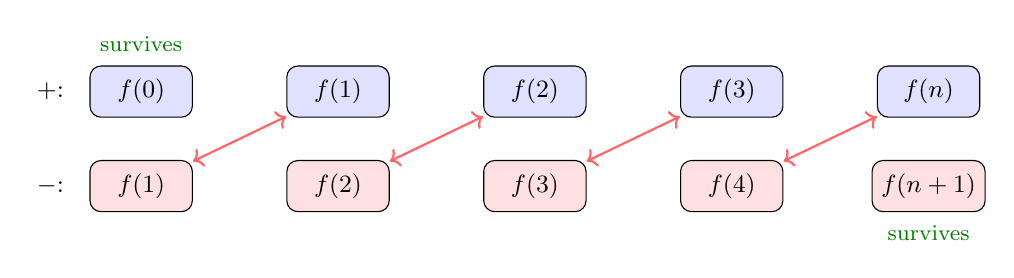
\begin{tikzpicture}[every node/.style={font=\small}]
  \foreach \r/\v in {1/f(0),2/f(1),3/f(2),4/f(3),5/f(n)}{
    \node[draw,rounded corners,fill=blue!12,minimum width=1.3cm,minimum height=0.65cm]
      (p\r) at ({(\r-1)*2.5},0.6) {$\v$};
  }
  \foreach \r/\v in {1/f(1),2/f(2),3/f(3),4/f(4),5/{f(n+1)}}{
    \node[draw,rounded corners,fill=red!12,minimum width=1.3cm,minimum height=0.65cm]
      (m\r) at ({(\r-1)*2.5},-0.6) {$\v$};
  }
  \node[left=0.2cm of p1]{$+$:};
  \node[left=0.2cm of m1]{$-$:};
  \foreach \a/\b in {2/1,3/2,4/3,5/4}{
    \draw[<->,thick,red!60] (m\b)--(p\a);
  }
  \node[below=0.05cm of m5,font=\footnotesize,green!50!black]{survives};
  \node[above=0.05cm of p1,font=\footnotesize,green!50!black]{survives};
\end{tikzpicture}
\end{center}
\noindent\textbf{Figure 1.} Cancellation pattern: only \(+f(0)\) and \(-f(n+1)\) survive (or equivalently \(f(n)-f(0)\) depending on orientation).

\subsection{Worked Examples}

\begin{example}{$\displaystyle\sumr \frac{1}{r(r+1)}$ via partial fractions}{}
\[
  \frac{1}{r(r+1)}=\frac{1}{r}-\frac{1}{r+1} = f(r-1)-f(r),\quad f(r)=\frac{1}{r+1}.
\]
\[
  \sumr\frac{1}{r(r+1)} = f(0)-f(n) = 1-\frac{1}{n+1} = \frac{n}{n+1}.
\]
As \(n\to\infty\), sum \(\to 1\).
\end{example}

\begin{example}{$\displaystyle\sumr r(r+1)$ via method of differences}{}
Note \(r(r+1)(r+2)-(r-1)r(r+1)=3r(r+1)\). So
\[
  \sumr r(r+1) = \frac{1}{3}\bigl[n(n+1)(n+2)-0\bigr]=\frac{n(n+1)(n+2)}{3}.
\]
\end{example}

% ─────────────────────────────────────────────────────────────────────────────
\section{Converging Series}

\begin{definition}
The \(n\)-th partial sum is \(S_n=\sumr a_r\). A series \emph{converges} if
\(\lim_{n\to\infty}S_n = L\in\R\); otherwise it \emph{diverges}.
\end{definition}

\begin{result}{Necessary condition}{}
If \(\sum a_r\) converges, then \(a_r\to 0\).
\end{result}

\begin{result}{Geometric series}{}
\(\ds\sum_{r=0}^{\infty}ar^k = \dfrac{a}{1-r}\) provided \(|r|<1\); diverges if \(|r|\geq1\).
\end{result}

\vspace{6pt}
\begin{center}
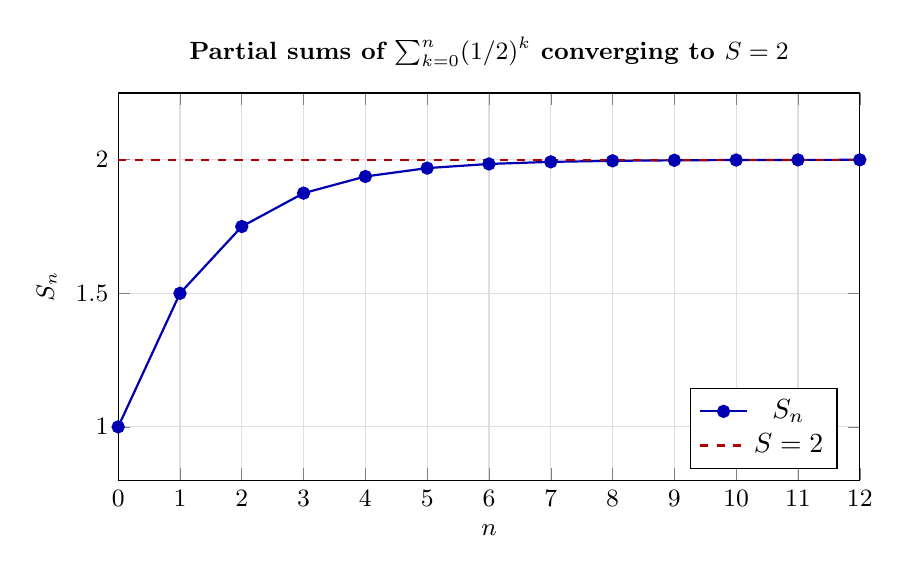
\begin{tikzpicture}
\begin{axis}[
  width=11cm,height=6.5cm,
  xlabel={$n$},ylabel={$S_n$},
  title={Partial sums of $\sum_{k=0}^n(1/2)^k$ converging to $S=2$},
  xmin=0,xmax=12,ymin=0.8,ymax=2.25,
  xtick={0,1,...,12},grid=major,
  grid style={draw=gray!25},
  legend pos=south east,
  tick label style={font=\small},label style={font=\small},
  title style={font=\small\bfseries}]
  \addplot[mark=*,mark size=2pt,blue!70!black,thick] coordinates {
    (0,1)(1,1.5)(2,1.75)(3,1.875)(4,1.9375)(5,1.96875)
    (6,1.984375)(7,1.9921875)(8,1.99609375)(9,1.998046875)
    (10,1.9990234375)(11,1.99951171875)(12,1.999755859375)};
  \addlegendentry{$S_n$}
  \addplot[dashed,red!70!black,thick,domain=0:12]{2};
  \addlegendentry{$S=2$}
\end{axis}
\end{tikzpicture}
\end{center}
\noindent\textbf{Figure 2.} Partial sums of a geometric series approaching the limit \(S=2\).

% ─────────────────────────────────────────────────────────────────────────────
% EXERCISES -- CHAPTER 3
% ─────────────────────────────────────────────────────────────────────────────
\exsection{Chapter 3 --- Summation of Series}
\resetQ

\begin{tcolorbox}[basic, title={\color{basiccol}\bfseries Basic}]

\Q{Evaluate using standard results: (a)~$\sumr r$;\; (b)~$\sumr r^2$;\; (c)~$\sumr r^3$;\; (d)~$\sum_{r=1}^{10}r$;\; (e)~$\sum_{r=1}^{6}r^2$.\mks{5}}

\Q{Find closed forms for: (a)~$\sumr(3r-1)$;\; (b)~$\sumr(2r^2+5)$;\; (c)~$\sumr(r^2-r+1)$. Factorise fully.\mks{6}}

\Q{Show that $3+6+12+\cdots+3\cdot2^{n-1}=3(2^n-1)$ and verify for $n=4$.\mks{4}}

\Q{A geometric series has $a=5$, $r=3/5$. Find $S_n$, $S_\infty$, and the least $n$ such that $S_\infty-S_n<0.01$.\mks{6}}

\Q{Show by writing out terms for $n=5$ that $\sum_{r=1}^{n}[f(r)-f(r-1)]=f(n)-f(0)$. Hence find $\sumr(2r-1)$ using $f(r)=r^2$.\mks{4}}

\end{tcolorbox}

\vspace{8pt}

\begin{tcolorbox}[medium, title={\color{medcol}\bfseries Medium}]

\Q{Find $\sumr r(r+1)(r+2)$ in fully factorised form.\mks{6}}

\Q{Using partial fractions, find $\sumr\dfrac{1}{(2r-1)(2r+1)}$ and state its sum to infinity.\mks{7}}

\Q{(a) Show $f(r)-f(r-1)=2r$ for $f(r)=r(r+1)$.\ \ (b) Derive $\sumr r=\tfrac{n(n+1)}{2}$.\ \ (c) Show $\sumr r(r+1)=\tfrac{n(n+1)(n+2)}{3}$.\mks{9}}

\Q{Show $\sumr r\cdot2^r=(n-1)\cdot2^{n+1}+2$ using the method of differences.\mks{7}}

\Q{Given $S_n=\dfrac{3n}{n+2}$, find $u_n$ for $n\geq2$, write down $u_1$, and determine convergence.\mks{6}}

\end{tcolorbox}

\vspace{8pt}

\begin{tcolorbox}[hard, title={\color{hardcol}\bfseries Hard}]

\Q{Prove $\sumr r^2=\dfrac{n(n+1)(2n+1)}{6}$ by method of differences and hence evaluate $\sum_{r=n+1}^{2n}r^2$.\mks{9}}

\Q{Find $A$ such that $f(r)-f(r+1)=\dfrac{1}{r(r+1)(r+2)(r+3)}$ where $f(r)=\dfrac{A}{r(r+1)(r+2)}$. Hence sum the series and find $S_\infty$.\mks{10}}

\Q{Prove $\left(\sumr r\right)^2=\sumr r^3$ and verify $\sumr r^3-\sum_{r=1}^{n-1}r^3=n^3$.\mks{8}}

\Q{Express $\dfrac{r^2+r-1}{r(r+1)(r+2)}$ in partial fractions. Identify the telescoping structure and find a closed form for the sum.\mks{11}}

\Q{Partial sums satisfy $3S_n-5S_{n-1}=8\cdot3^n$, $S_1=12$. Find $a_n$ in closed form and determine convergence.\mks{10}}

\end{tcolorbox}

\vspace{8pt}

\begin{tcolorbox}[explore, title={\color{explorecol}\bfseries Exploration (Beyond Syllabus)}]

\Q{\textbf{A rational cousin of the Basel problem.}
\begin{enumerate}[label=(\alph*),itemsep=4pt]
  \item Show $\dfrac{1}{r^2-1}=\dfrac{1}{2}\!\left(\dfrac{1}{r-1}-\dfrac{1}{r+1}\right)$ for $r\geq2$.\hfill\textit{[2]}
  \item Write out the telescoping structure for $\sum_{r=2}^{n}\dfrac{1}{r^2-1}$ explicitly.\hfill\textit{[3]}
  \item Show $\sum_{r=2}^{n}\dfrac{1}{r^2-1}=\dfrac{1}{2}\!\left[1+\tfrac{1}{2}-\tfrac{1}{n}-\tfrac{1}{n+1}\right]$ and deduce $\sum_{r=2}^\infty\dfrac{1}{r^2-1}=\dfrac{3}{4}$.\hfill\textit{[7]}
  \item Use a comparison argument to show $\sumt\dfrac{1}{r^2}<\dfrac{7}{4}$. Reflect on why the telescoping method cannot yield the Basel sum $\pi^2/6$.\hfill\textit{[5]}
\end{enumerate}\mks{17}}

\Q{\textbf{Factorial telescoping and an exponential connection.}
\begin{enumerate}[label=(\alph*),itemsep=4pt]
  \item Compute $E_n=\sum_{k=0}^{n}\dfrac{1}{k!}$ for $n=0,1,2,3,4$.\hfill\textit{[2]}
  \item Show the tail $T_n=e-E_n\leq\dfrac{1}{n!\cdot n}$ by bounding via a geometric series.\hfill\textit{[5]}
  \item Using $(k+1)!\,E_k - k!\,E_{k-1}$, derive $\sum_{k=1}^{n}k\cdot k!=(n+1)!-1$.\hfill\textit{[7]}
  \item Verify for $n=1,2,3$ and hence find $\sumt\dfrac{k\cdot k!}{(k+2)!}$.\hfill\textit{[7]}
\end{enumerate}\mks{21}}

\end{tcolorbox}


% ══════════════════════════════════════════════════════════════════════════════
%  CHAPTER 4 -- MATRICES 1
% ══════════════════════════════════════════════════════════════════════════════
\chapterbanner{4}{Matrices 1}

A \emph{matrix} is a rectangular array of numbers. This chapter covers operations, inverses, determinants, and geometric transformations represented by \(2\times2\) and \(3\times3\) matrices.

% ─────────────────────────────────────────────────────────────────────────────
\section{Matrix Operations}

\subsection{Addition, Scalar Multiplication, and Matrix Multiplication}

\begin{result}{}{}
For matrices of compatible sizes:
\[
  (A+B)_{ij}=A_{ij}+B_{ij},\quad
  (kA)_{ij}=kA_{ij},\quad
  (AB)_{ij}=\sum_k A_{ik}B_{kj}.
\]
Matrix multiplication is \emph{associative} and \emph{distributive}, but in general \textbf{not commutative}: \(AB\neq BA\).
\end{result}

\begin{example}{Multiply $A=\begin{pmatrix}1&2\\3&4\end{pmatrix}$ and $B=\begin{pmatrix}0&1\\-1&2\end{pmatrix}$}{}
\[
  AB = \begin{pmatrix}1\cdot0+2\cdot(-1) & 1\cdot1+2\cdot2\\ 3\cdot0+4\cdot(-1) & 3\cdot1+4\cdot2\end{pmatrix}
     = \begin{pmatrix}-2 & 5\\ -4 & 11\end{pmatrix}.
\]
\[
  BA = \begin{pmatrix}3&4\\5&6\end{pmatrix} \neq AB. \quad\text{(Non-commutative.)}
\]
\end{example}

\subsection{Transpose and Special Matrices}

\begin{result}{}{}
The \emph{transpose} \(A^T\) is obtained by reflecting across the main diagonal: \((A^T)_{ij}=A_{ji}\).
\begin{itemize}[nosep]
  \item \emph{Symmetric}: \(A^T=A\).
  \item \emph{Identity} \(I\): \(IA=AI=A\) for all compatible \(A\).
  \item \emph{Zero matrix} \(O\): all entries zero.
\end{itemize}
\end{result}

% ─────────────────────────────────────────────────────────────────────────────
\section{The Inverse Matrix}

\begin{definition}
The \emph{inverse} of a square matrix \(A\) is the matrix \(A^{-1}\) (if it exists) such that
\(AA^{-1}=A^{-1}A=I\).
\end{definition}

\begin{result}{Inverse of a $2\times2$ matrix}{}
\[
  A = \begin{pmatrix}a&b\\c&d\end{pmatrix},\quad
  A^{-1} = \frac{1}{ad-bc}\begin{pmatrix}d&-b\\-c&a\end{pmatrix},\quad ad-bc\neq 0.
\]
\end{result}

\subsubsection*{Derivation}
Let \(A^{-1}=\dfrac{1}{\det A}\begin{pmatrix}d&-b\\-c&a\end{pmatrix}\). Then:
\[
  AA^{-1}=\frac{1}{ad-bc}\begin{pmatrix}a&b\\c&d\end{pmatrix}\begin{pmatrix}d&-b\\-c&a\end{pmatrix}
  =\frac{1}{ad-bc}\begin{pmatrix}ad-bc&0\\0&ad-bc\end{pmatrix}=I. \qquad\square
\]

\begin{result}{Properties of inverses}{}
\[
  (AB)^{-1}=B^{-1}A^{-1},\quad (A^T)^{-1}=(A^{-1})^T,\quad (A^{-1})^{-1}=A.
\]
\end{result}

\begin{example}{Find $A^{-1}$ for $A=\begin{pmatrix}3&1\\5&2\end{pmatrix}$}{}
\(\det A=6-5=1\). So \(A^{-1}=\begin{pmatrix}2&-1\\-5&3\end{pmatrix}\).
Check: \(AA^{-1}=\begin{pmatrix}1&0\\0&1\end{pmatrix}\). \checkmark
\end{example}

% ─────────────────────────────────────────────────────────────────────────────
\section{Determinants}

\subsection{\(2\times2\) Determinant}

\[
  \det\begin{pmatrix}a&b\\c&d\end{pmatrix} = ad-bc.
\]

\subsection{\(3\times3\) Determinant --- Cofactor Expansion}

\begin{result}{}{}
Expanding along the first row:
\[
  \det\begin{pmatrix}a&b&c\\d&e&f\\g&h&i\end{pmatrix}
  = a(ei-fh)-b(di-fg)+c(dh-eg).
\]
\end{result}

\subsubsection*{Geometric meaning}

\(\det A\) equals the (signed) scale factor by which the matrix \(A\) multiplies areas (\(2\times2\)) or volumes (\(3\times3\)).  If \(\det A=0\), the transformation is \emph{singular} (collapses dimension) and \(A^{-1}\) does not exist.

\begin{result}{Determinant properties}{}
\[
  \det(AB)=\det A\cdot\det B,\quad \det(A^{-1})=\frac{1}{\det A},\quad \det(A^T)=\det A.
\]
\end{result}

\begin{example}{$3\times3$ determinant}{}
\[
  \det\begin{pmatrix}2&1&-1\\0&3&2\\1&-1&4\end{pmatrix}
  = 2(12-(-2))-1(0-2)+(-1)(0-3) = 2(14)-1(-2)+(-1)(-3)=28+2+3=33.
\]
\end{example}

% ─────────────────────────────────────────────────────────────────────────────
\section{Matrix Transformations}

Common \(2\times2\) transformation matrices (acting on column vectors \(\begin{pmatrix}x\\y\end{pmatrix}\)):

\begin{result}{}{}
\renewcommand{\arraystretch}{1.6}
\begin{center}
\begin{tabular}{ll}
\toprule
Transformation & Matrix \\
\midrule
Rotation by \(\theta\) anticlockwise about origin
  & $\begin{pmatrix}\cos\theta & -\sin\theta\\ \sin\theta & \cos\theta\end{pmatrix}$ \\[6pt]
Reflection in \(y=x\)
  & $\begin{pmatrix}0&1\\1&0\end{pmatrix}$ \\[6pt]
Reflection in \(x\)-axis
  & $\begin{pmatrix}1&0\\0&-1\end{pmatrix}$ \\[6pt]
Enlargement scale factor \(k\)
  & $\begin{pmatrix}k&0\\0&k\end{pmatrix}$ \\[6pt]
Shear (factor \(k\)) parallel to \(x\)-axis
  & $\begin{pmatrix}1&k\\0&1\end{pmatrix}$ \\
\bottomrule
\end{tabular}
\end{center}
\end{result}

\begin{example}{Find the image of triangle with vertices $O(0,0)$, $A(1,0)$, $B(0,1)$ under $M=\begin{pmatrix}2&1\\0&3\end{pmatrix}$}{}
\[
  MO=\begin{pmatrix}0\\0\end{pmatrix},\quad
  MA=\begin{pmatrix}2\\0\end{pmatrix},\quad
  MB=\begin{pmatrix}1\\3\end{pmatrix}.
\]
Area of image \(= |\det M|\times\) area of original \(= 6\times\frac{1}{2}=3\).
\end{example}

% TikZ diagram -- transformation
\vspace{6pt}
\begin{center}
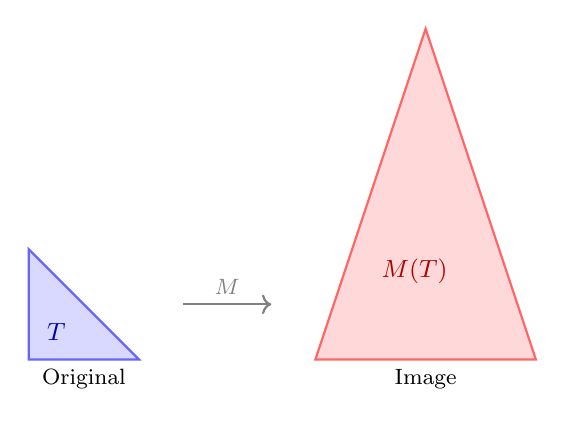
\begin{tikzpicture}[scale=1.4]
  % Original triangle
  \fill[blue!15,draw=blue!60,thick] (0,0)--(1,0)--(0,1)--cycle;
  \node[blue!70!black] at (0.25,0.25) {\small$T$};
  \node[below,font=\footnotesize] at (0.5,0) {Original};
  % Arrow
  \draw[->,thick,gray] (1.4,0.5) -- (2.2,0.5) node[midway,above,font=\footnotesize]{$M$};
  % Image triangle
  \fill[red!15,draw=red!60,thick] (2.6,0)--(4.6,0)--(3.6,3)--cycle;
  \node[red!70!black] at (3.5,0.8) {\small$M(T)$};
  \node[below,font=\footnotesize] at (3.6,0) {Image};
\end{tikzpicture}
\end{center}
\noindent\textbf{Figure 3.} A unit triangle mapped by \(M=\begin{pmatrix}2&1\\0&3\end{pmatrix}\). Area scales by \(|\det M|=6\).

% ─────────────────────────────────────────────────────────────────────────────
% EXERCISES -- CHAPTER 4
% ─────────────────────────────────────────────────────────────────────────────
\exsection{Chapter 4 --- Matrices 1}
\resetQ

\begin{tcolorbox}[basic, title={\color{basiccol}\bfseries Basic}]

\Q{Given $A=\begin{pmatrix}2&-1\\3&4\end{pmatrix}$ and $B=\begin{pmatrix}1&5\\0&-2\end{pmatrix}$, find: (a)~$A+B$; (b)~$AB$; (c)~$BA$; (d)~$A^2$.\mks{6}}

\Q{Find the inverse of each matrix, or state that it is singular:
(a)~$\begin{pmatrix}4&3\\2&1\end{pmatrix}$;\quad
(b)~$\begin{pmatrix}6&3\\4&2\end{pmatrix}$;\quad
(c)~$\begin{pmatrix}5&2\\3&1\end{pmatrix}$.\mks{6}}

\Q{Evaluate: $\det\begin{pmatrix}3&-1\\2&5\end{pmatrix}$ and $\det\begin{pmatrix}1&2&3\\0&4&5\\1&0&2\end{pmatrix}$.\mks{5}}

\Q{Write down the $2\times2$ matrix for: (a) rotation by $90^\circ$ anticlockwise; (b) reflection in the $y$-axis; (c) enlargement scale factor 3.\mks{4}}

\Q{Use matrix multiplication to solve the system $2x-y=5$, $x+3y=-1$ by writing it as $A\mathbf{x}=\mathbf{b}$ and computing $\mathbf{x}=A^{-1}\mathbf{b}$.\mks{5}}

\end{tcolorbox}

\vspace{8pt}

\begin{tcolorbox}[medium, title={\color{medcol}\bfseries Medium}]

\Q{Show that if $A^2=A$ (idempotent), then $\det A = 0$ or $\det A = 1$, and give an example of each.\mks{6}}

\Q{The transformation $T_1$ is a rotation by $60^\circ$ and $T_2$ is a reflection in the line $y=x\tan30^\circ$. Find the matrix of $T_2\circ T_1$ and describe the combined transformation geometrically.\mks{8}}

\Q{Prove that for invertible $A$ and $B$: (a) $(AB)^{-1}=B^{-1}A^{-1}$; (b) $\det(AB)=\det A\cdot\det B$.\mks{8}}

\Q{Find all values of $k$ for which $M=\begin{pmatrix}k&2&0\\1&k&1\\0&3&k\end{pmatrix}$ is singular.\mks{7}}

\Q{A transformation $T$ maps the unit square to a parallelogram of area 10. Given that $T$ has matrix $\begin{pmatrix}a&2\\1&a\end{pmatrix}$, find the possible values of $a$.\mks{5}}

\end{tcolorbox}

\vspace{8pt}

\begin{tcolorbox}[hard, title={\color{hardcol}\bfseries Hard}]

\Q{Prove the Cayley--Hamilton theorem for $2\times2$ matrices: every matrix satisfies its own characteristic equation $\det(A-\lambda I)=0$. That is, if $\lambda^2-(\text{tr}\,A)\lambda+\det A=0$ is the characteristic equation, show $A^2-(\text{tr}\,A)A+(\det A)I=O$.\mks{8}}

\Q{Let $A=\begin{pmatrix}\cos\theta&-\sin\theta\\\sin\theta&\cos\theta\end{pmatrix}$. Prove by induction that $A^n=\begin{pmatrix}\cos n\theta&-\sin n\theta\\\sin n\theta&\cos n\theta\end{pmatrix}$.\mks{8}}

\Q{The matrix $M=\begin{pmatrix}a&b\\c&d\end{pmatrix}$ represents a transformation that maps the line $y=2x$ to itself and the line $y=x$ to itself. Find all possible matrices $M$ (up to a scalar multiple).\mks{9}}

\Q{Show that if $A$ and $B$ are both $n\times n$ invertible matrices and $AB=BA$, then $(A+B)^{-1}$ exists iff $A+B$ is invertible, and find $(A+B)^{-1}$ in terms of $A^{-1}$ and $B^{-1}$ when $A+B$ is invertible.\mks{8}}

\Q{A matrix $R$ satisfies $R^T=R^{-1}$ (orthogonal matrix). Prove: (a) $|\det R|=1$; (b) the eigenvalues of $R$ have modulus 1; (c) if $R$ is $2\times2$ real and $\det R=1$, then $R$ is a rotation matrix.\mks{9}}

\end{tcolorbox}

\vspace{8pt}

\begin{tcolorbox}[explore, title={\color{explorecol}\bfseries Exploration (Beyond Syllabus)}]

\Q{\textbf{Matrix exponentials and the connection to transformations.}

For a square matrix $A$, define $e^A = I + A + \dfrac{A^2}{2!} + \dfrac{A^3}{3!}+\cdots$
\begin{enumerate}[label=(\alph*),itemsep=4pt]
  \item Let $J=\begin{pmatrix}0&-1\\1&0\end{pmatrix}$. Show $J^2=-I$, $J^3=-J$, $J^4=I$, establishing the period-4 cycle.\hfill\textit{[3]}
  \item Using the cycle, show $e^{\theta J}=\begin{pmatrix}\cos\theta&-\sin\theta\\\sin\theta&\cos\theta\end{pmatrix}$ by grouping even and odd terms of the series.\hfill\textit{[6]}
  \item Deduce that $e^{\theta J}\cdot e^{\phi J}=e^{(\theta+\phi)J}$ and interpret geometrically.\hfill\textit{[3]}
\end{enumerate}\mks{12}}

\Q{\textbf{Determinants and signed areas --- a generalisation.}

\begin{enumerate}[label=(\alph*),itemsep=4pt]
  \item Prove that the (signed) area of a triangle with vertices $(x_1,y_1),(x_2,y_2),(x_3,y_3)$ is $\dfrac{1}{2}\det\begin{pmatrix}x_2-x_1&x_3-x_1\\y_2-y_1&y_3-y_1\end{pmatrix}$.\hfill\textit{[4]}
  \item Hence express the area of a polygon with $n$ vertices as a sum of determinants (the shoelace formula).\hfill\textit{[4]}
  \item Prove that three points are collinear iff $\det\begin{pmatrix}x_1&y_1&1\\x_2&y_2&1\\x_3&y_3&1\end{pmatrix}=0$.\hfill\textit{[4]}
\end{enumerate}\mks{12}}

\end{tcolorbox}


% ══════════════════════════════════════════════════════════════════════════════
%  CHAPTER 5 -- POLAR COORDINATES
% ══════════════════════════════════════════════════════════════════════════════
\chapterbanner{5}{Polar Coordinates}

Polar coordinates \((r,\theta)\) locate a point by its distance from the origin (pole) and angle from the initial line (positive \(x\)-axis). They are particularly effective for curves with rotational or radial symmetry.

% ─────────────────────────────────────────────────────────────────────────────
\section{The Polar System}

\subsection{Conversion Between Polar and Cartesian}

\begin{result}{}{}
\[
  x = r\cos\theta,\quad y = r\sin\theta,\quad r = \sqrt{x^2+y^2},\quad \theta=\arctan\!\left(\frac{y}{x}\right).
\]
By convention \(r\geq 0\) and \(\theta\in(-\pi,\pi]\) or \([0,2\pi)\).
\end{result}

\subsection{Common Polar Curves}

\begin{result}{}{}
\renewcommand{\arraystretch}{1.5}
\begin{center}
\begin{tabular}{lll}
\toprule
Name & Equation & Notes \\
\midrule
Circle (centre $O$) & $r=a$ & radius $a$ \\
Circle through $O$ & $r=2a\cos\theta$ & centre $(a,0)$ \\
Cardioid & $r=a(1+\cos\theta)$ & heart-shaped \\
Rose (4 petals) & $r=a\cos2\theta$ & petals at $\theta=0,\tfrac{\pi}{2},\pi,\tfrac{3\pi}{2}$ \\
Lemniscate & $r^2=a^2\cos2\theta$ & figure-of-eight \\
Archimedean spiral & $r=a\theta$ & \\
\bottomrule
\end{tabular}
\end{center}
\end{result}

\begin{example}{Sketch $r=2(1+\cos\theta)$}{}
At \(\theta=0\): \(r=4\) (rightmost point). At \(\theta=\pi/2\): \(r=2\). At \(\theta=\pi\): \(r=0\) (cusp at origin). The curve is a cardioid symmetric about the initial line.
\end{example}

\vspace{6pt}
\begin{center}
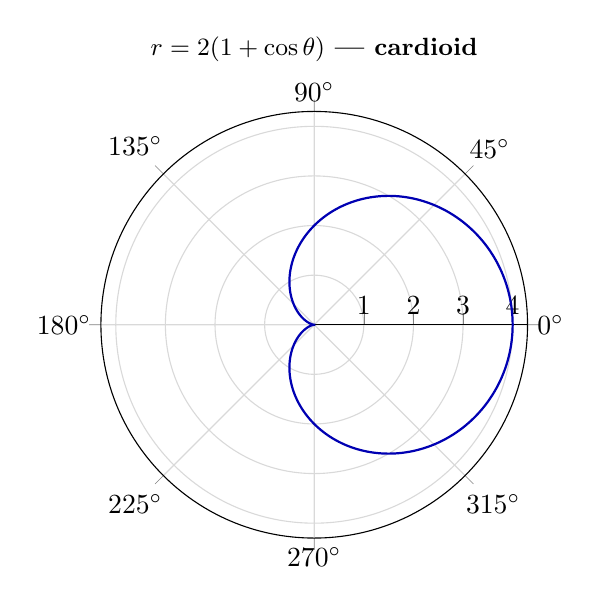
\begin{tikzpicture}
\begin{polaraxis}[
  width=7cm, xtick={0,45,...,315},
  xticklabel={\pgfmathparse{\tick}\pgfmathprintnumber{\pgfmathresult}$^\circ$},
  ymin=0,ymax=4.3,ytick={1,2,3,4},
  grid=both, grid style={draw=gray!30},
  title={$r=2(1+\cos\theta)$ --- cardioid},
  title style={font=\small\bfseries}]
  \addplot[domain=0:360,samples=300,blue!70!black,thick]
    {2*(1+cos(x))};
\end{polaraxis}
\end{tikzpicture}
\end{center}
\noindent\textbf{Figure 4.} Cardioid \(r=2(1+\cos\theta)\).

% ─────────────────────────────────────────────────────────────────────────────
\section{Applications of Polar Coordinates}

\subsection{Area in Polar Coordinates}

\begin{result}{}{}
The area enclosed by the curve \(r=f(\theta)\) between \(\theta=\alpha\) and \(\theta=\beta\) is
\[
  A = \frac{1}{2}\int_\alpha^\beta r^2\,d\theta.
\]
\end{result}

\subsubsection*{Derivation}
A thin sector of angle \(d\theta\) and radius \(r\) has area \(\approx\dfrac{1}{2}r^2\,d\theta\). Integrating gives the result. \(\square\)

\begin{example}{Area enclosed by the cardioid $r=a(1+\cos\theta)$}{}
By symmetry integrate from \(0\) to \(\pi\) and double:
\[
\begin{aligned}
  A &= 2\cdot\frac{1}{2}\int_0^\pi a^2(1+\cos\theta)^2\,d\theta
     = a^2\int_0^\pi(1+2\cos\theta+\cos^2\theta)\,d\theta \\[4pt]
    &= a^2\int_0^\pi\!\left(1+2\cos\theta+\frac{1+\cos2\theta}{2}\right)d\theta \\[4pt]
    &= a^2\left[\theta+2\sin\theta+\frac{\theta}{2}+\frac{\sin2\theta}{4}\right]_0^\pi
     = a^2\cdot\frac{3\pi}{2} = \frac{3\pi a^2}{2}.
\end{aligned}
\]
\end{example}

\begin{example}{Area of one petal of $r=\cos2\theta$}{}
One petal lies between \(\theta=-\pi/4\) and \(\theta=\pi/4\):
\[
  A=\frac{1}{2}\int_{-\pi/4}^{\pi/4}\cos^2 2\theta\,d\theta
   =\frac{1}{2}\int_{-\pi/4}^{\pi/4}\frac{1+\cos4\theta}{2}\,d\theta
   =\frac{1}{4}\left[\theta+\frac{\sin4\theta}{4}\right]_{-\pi/4}^{\pi/4}=\frac{\pi}{8}.
\]
\end{example}

% ─────────────────────────────────────────────────────────────────────────────
% EXERCISES -- CHAPTER 5
% ─────────────────────────────────────────────────────────────────────────────
\exsection{Chapter 5 --- Polar Coordinates}
\resetQ

\begin{tcolorbox}[basic, title={\color{basiccol}\bfseries Basic}]

\Q{Convert to Cartesian: (a) $(3, \pi/3)$; (b) $(2, 3\pi/4)$; (c) $(1, -\pi/6)$.\mks{4}}

\Q{Convert to polar ($r>0$, $\theta\in(-\pi,\pi]$): (a) $(1,\sqrt{3})$; (b) $(-2,2)$; (c) $(0,-5)$.\mks{4}}

\Q{Sketch the curves: (a) $r=3$; (b) $\theta=\pi/4$; (c) $r=4\sin\theta$. Label key points on each.\mks{5}}

\Q{Show that $r=2\cos\theta$ is a circle and find its Cartesian equation, centre, and radius.\mks{4}}

\Q{Find the area enclosed by $r=2$ between $\theta=0$ and $\theta=\pi/2$. Verify by geometry.\mks{4}}

\end{tcolorbox}

\vspace{8pt}

\begin{tcolorbox}[medium, title={\color{medcol}\bfseries Medium}]

\Q{Sketch the cardioid $r=1+\sin\theta$, identifying the cusp and maximum $r$. Find the total enclosed area.\mks{8}}

\Q{Find the area enclosed by the curve $r^2=4\cos2\theta$. State the domain of $\theta$ for which the curve exists.\mks{7}}

\Q{Find the points of intersection of $r=2$ and $r=3-2\cos\theta$. Hence find the area of the region inside $r=2$ but outside $r=3-2\cos\theta$.\mks{9}}

\Q{Show that the length of the arc of $r=a\theta$ from $\theta=0$ to $\theta=\Theta$ is $\dfrac{a}{2}\left[\Theta\sqrt{1+\Theta^2}+\ln\!\left(\Theta+\sqrt{1+\Theta^2}\right)\right]$.\mks{8}}

\Q{For the lemniscate $r^2=a^2\cos2\theta$, find the total area and the Cartesian equation.\mks{6}}

\end{tcolorbox}

\vspace{8pt}

\begin{tcolorbox}[hard, title={\color{hardcol}\bfseries Hard}]

\Q{The curve $r=a(1+\cos\theta)$ and the circle $r=\dfrac{3a}{2}$ intersect. Find: (a) their intersection points; (b) the area of the region inside the circle but outside the cardioid; (c) the area inside the cardioid but outside the circle.\mks{12}}

\Q{Prove that the area between the two loops of the limacon $r=1+2\cos\theta$ (the region inside the outer loop but outside the inner loop) is $\pi+\dfrac{3\sqrt{3}}{2}$.\mks{10}}

\Q{Show that the curve $r=\sec\theta+2$ has a vertical asymptote. Find the asymptote and sketch the curve.\mks{8}}

\Q{By converting to Cartesian coordinates, show that the spiral $r=e^\theta$ has the property that the angle between the tangent and the radius vector is constant. Find this angle.\mks{9}}

\Q{Find the area common to the two circles $r=2\sin\theta$ and $r=2\cos\theta$, giving your answer in exact form.\mks{8}}

\end{tcolorbox}

\vspace{8pt}

\begin{tcolorbox}[explore, title={\color{explorecol}\bfseries Exploration (Beyond Syllabus)}]

\Q{\textbf{Arc length in polar form.}

The arc length of a polar curve is $L=\int_\alpha^\beta\sqrt{r^2+\left(\dfrac{dr}{d\theta}\right)^2}\,d\theta$.
\begin{enumerate}[label=(\alph*),itemsep=4pt]
  \item Derive this formula from the Cartesian arc length formula $L=\int\sqrt{\left(\dfrac{dx}{d\theta}\right)^2+\left(\dfrac{dy}{d\theta}\right)^2}\,d\theta$ using $x=r\cos\theta$, $y=r\sin\theta$.\hfill\textit{[5]}
  \item Use the formula to find the perimeter of the cardioid $r=a(1+\cos\theta)$. [\textit{Answer: $8a$.}]\hfill\textit{[7]}
  \item Show that for the Archimedean spiral $r=a\theta$, the arc length from $\theta=0$ to $\theta=\Theta$ can be expressed as an integral and evaluate it using the substitution $\theta=\sinh t$.\hfill\textit{[6]}
\end{enumerate}\mks{18}}

\Q{\textbf{Polar curves and complex numbers.}

Every point $(r,\theta)$ in the plane corresponds to the complex number $z=re^{i\theta}=r(\cos\theta+i\sin\theta)$.
\begin{enumerate}[label=(\alph*),itemsep=4pt]
  \item Show that the cardioid $r=a(1+\cos\theta)$ in polar form corresponds, in complex notation, to the image of the unit circle under the map $w=a\left(z+\dfrac{1}{z}+2\right)/2$ (where $|z|=1$).\hfill\textit{[5]}
  \item A four-petalled rose is given by $r=\cos2\theta$. Write $r^2=r\cos2\theta=r\cos^2\theta-r\sin^2\theta$ and hence find its Cartesian equation in the form $(x^2+y^2)^n=f(x,y)$.\hfill\textit{[4]}
  \item For the curve $r^n=a^n\cos n\theta$, show that the total area is $\dfrac{\pi a^2}{2}$ for all $n\in\mathbb{N}$ with $n\geq2$.\hfill\textit{[5]}
\end{enumerate}\mks{14}}

\end{tcolorbox}

% ══════════════════════════════════════════════════════════════════════════════
%  CHAPTER 6 -- VECTORS
% ══════════════════════════════════════════════════════════════════════════════
\chapterbanner{6}{Vectors}

This chapter extends vectors to three dimensions, introducing the vector (cross) product, equations of lines, and equations of planes.

% ─────────────────────────────────────────────────────────────────────────────
\section{The Vector Product}

\begin{definition}
The \emph{vector product} (cross product) of \(\mathbf{a},\mathbf{b}\in\R^3\) is
\[
  \mathbf{a}\times\mathbf{b} = |\mathbf{a}||\mathbf{b}|\sin\theta\,\hat{\mathbf{n}},
\]
where \(\theta\) is the angle between them and \(\hat{\mathbf{n}}\) is the unit normal (right-hand rule).
\end{definition}

\begin{result}{Component form}{}
\[
  \mathbf{a}\times\mathbf{b}
  = \det\begin{pmatrix}\mathbf{i}&\mathbf{j}&\mathbf{k}\\a_1&a_2&a_3\\b_1&b_2&b_3\end{pmatrix}
  = \begin{pmatrix}a_2b_3-a_3b_2\\ a_3b_1-a_1b_3\\ a_1b_2-a_2b_1\end{pmatrix}.
\]
\end{result}

\begin{result}{Properties}{}
\begin{itemize}[nosep]
  \item Anti-commutative: \(\mathbf{a}\times\mathbf{b}=-\mathbf{b}\times\mathbf{a}\).
  \item \(\mathbf{a}\times\mathbf{a}=\mathbf{0}\).
  \item \(|\mathbf{a}\times\mathbf{b}|=|\mathbf{a}||\mathbf{b}|\sin\theta\) = area of parallelogram spanned by \(\mathbf{a},\mathbf{b}\).
  \item \(\mathbf{a}\times\mathbf{b}=\mathbf{0}\iff\mathbf{a}\parallel\mathbf{b}\).
\end{itemize}
\end{result}

\begin{example}{Find $\mathbf{a}\times\mathbf{b}$ for $\mathbf{a}=(2,1,-1)$, $\mathbf{b}=(1,3,2)$}{}
\[
  \mathbf{a}\times\mathbf{b}=\begin{vmatrix}\mathbf{i}&\mathbf{j}&\mathbf{k}\\2&1&-1\\1&3&2\end{vmatrix}
  = \mathbf{i}(2+3)-\mathbf{j}(4+1)+\mathbf{k}(6-1)
  = (5,-5,5).
\]
Area of parallelogram \(= |(5,-5,5)| = 5\sqrt{3}\).
\end{example}

% ─────────────────────────────────────────────────────────────────────────────
\section{Vector Equation of a Line}

\begin{result}{}{}
The line through point \(\mathbf{a}\) with direction \(\mathbf{d}\) has vector equation
\[
  \mathbf{r} = \mathbf{a} + t\mathbf{d},\quad t\in\R.
\]
In component (parametric) form with \(\mathbf{a}=(a_1,a_2,a_3)\) and \(\mathbf{d}=(d_1,d_2,d_3)\):
\[
  \frac{x-a_1}{d_1}=\frac{y-a_2}{d_2}=\frac{z-a_3}{d_3}=t\quad\text{(Cartesian/symmetric form)}.
\]
\end{result}

\begin{example}{Line through $A(1,2,-1)$ and $B(3,0,4)$}{}
Direction: \(\mathbf{d}=\overrightarrow{AB}=(2,-2,5)\).
\[
  \mathbf{r}=\begin{pmatrix}1\\2\\-1\end{pmatrix}+t\begin{pmatrix}2\\-2\\5\end{pmatrix},\quad
  \frac{x-1}{2}=\frac{y-2}{-2}=\frac{z+1}{5}.
\]
\end{example}

\subsection{Angle Between Two Lines}

The acute angle \(\theta\) between lines with directions \(\mathbf{d}_1,\mathbf{d}_2\):
\[
  \cos\theta = \frac{|\mathbf{d}_1\cdot\mathbf{d}_2|}{|\mathbf{d}_1||\mathbf{d}_2|}.
\]

% ─────────────────────────────────────────────────────────────────────────────
\section{Planes}

\subsection{Vector and Cartesian Equations}

\begin{result}{}{}
The plane through point \(\mathbf{a}\) with normal \(\mathbf{n}=(n_1,n_2,n_3)\):
\[
  \mathbf{n}\cdot\mathbf{r} = \mathbf{n}\cdot\mathbf{a} \iff n_1x+n_2y+n_3z=d,\quad d=\mathbf{n}\cdot\mathbf{a}.
\]
The plane through three non-collinear points \(A,B,C\):
\[
  \mathbf{n} = \overrightarrow{AB}\times\overrightarrow{AC}.
\]
\end{result}

\subsection{Distances}

\begin{result}{}{}
Distance from point \(P(\mathbf{p})\) to plane \(\mathbf{n}\cdot\mathbf{r}=d\):
\[
  \text{dist} = \frac{|\mathbf{n}\cdot\mathbf{p}-d|}{|\mathbf{n}|}.
\]
\end{result}

\begin{example}{Distance from $P(1,1,1)$ to $2x-y+2z=5$}{}
\[
  \text{dist}=\frac{|2-1+2-5|}{\sqrt{4+1+4}}=\frac{|-2|}{3}=\frac{2}{3}.
\]
\end{example}

\begin{example}{Find the equation of the plane through $A(1,0,0)$, $B(0,2,0)$, $C(0,0,3)$}{}
\[
  \overrightarrow{AB}=(-1,2,0),\quad\overrightarrow{AC}=(-1,0,3).
\]
\[
  \mathbf{n}=\overrightarrow{AB}\times\overrightarrow{AC}=(6,3,2).
\]
Plane: \(6x+3y+2z=6\) (check: \(A\) gives \(6\cdot1=6\).\;\checkmark)
\end{example}

% ─────────────────────────────────────────────────────────────────────────────
% EXERCISES -- CHAPTER 6
% ─────────────────────────────────────────────────────────────────────────────
\exsection{Chapter 6 --- Vectors}
\resetQ

\begin{tcolorbox}[basic, title={\color{basiccol}\bfseries Basic}]

\Q{Find $\mathbf{a}\times\mathbf{b}$ for: (a) $\mathbf{a}=(1,2,3)$, $\mathbf{b}=(4,5,6)$; (b) $\mathbf{a}=(2,-1,1)$, $\mathbf{b}=(1,3,-2)$. Verify $\mathbf{a}\cdot(\mathbf{a}\times\mathbf{b})=0$ in each case.\mks{6}}

\Q{Find the vector equation and Cartesian form of the line through $(2,-1,3)$ with direction $(1,4,-2)$.\mks{4}}

\Q{Find the equation of the plane with normal $(3,1,-2)$ passing through the point $(1,0,4)$.\mks{3}}

\Q{Find the distance from the point $(2,1,-3)$ to the plane $x-2y+2z=6$.\mks{4}}

\Q{Determine whether the lines $\mathbf{r}=(1,0,2)+t(2,1,-1)$ and $\mathbf{r}=(3,2,0)+s(1,-1,1)$ intersect. If so, find the intersection point.\mks{5}}

\end{tcolorbox}

\vspace{8pt}

\begin{tcolorbox}[medium, title={\color{medcol}\bfseries Medium}]

\Q{Find the equation of the plane through $A(1,2,3)$, $B(3,-1,2)$, $C(2,1,-1)$. Find the distance from the origin to this plane.\mks{8}}

\Q{Two planes are given by $\Pi_1: 2x-y+z=3$ and $\Pi_2: x+y-z=1$. Find: (a) the angle between them; (b) the vector equation of their line of intersection.\mks{9}}

\Q{Show that the lines $\dfrac{x-1}{2}=\dfrac{y-2}{3}=\dfrac{z-3}{4}$ and $\dfrac{x+1}{1}=\dfrac{y-1}{-1}=\dfrac{z}{2}$ are skew. Find the shortest distance between them.\mks{10}}

\Q{The points $A(2,0,1)$, $B(0,3,-1)$, $C(1,1,2)$, $D$ form a parallelogram. Find $D$ and the area of the parallelogram.\mks{7}}

\Q{A line $\ell$ has equation $\mathbf{r}=\mathbf{a}+t\mathbf{d}$. Show that the foot of the perpendicular from point $P$ to $\ell$ is at parameter $t^*=\dfrac{(\mathbf{p}-\mathbf{a})\cdot\mathbf{d}}{|\mathbf{d}|^2}$.\mks{5}}

\end{tcolorbox}

\vspace{8pt}

\begin{tcolorbox}[hard, title={\color{hardcol}\bfseries Hard}]

\Q{Prove the vector triple product identity $\mathbf{a}\times(\mathbf{b}\times\mathbf{c})=(\mathbf{a}\cdot\mathbf{c})\mathbf{b}-(\mathbf{a}\cdot\mathbf{b})\mathbf{c}$ by expanding in components.\mks{8}}

\Q{Using the scalar triple product $[\mathbf{a},\mathbf{b},\mathbf{c}]=\mathbf{a}\cdot(\mathbf{b}\times\mathbf{c})$, prove that four points $A,B,C,D$ are coplanar iff $[\overrightarrow{AB},\overrightarrow{AC},\overrightarrow{AD}]=0$. Test whether $(1,1,0),(2,0,1),(0,2,1),(3,1,2)$ are coplanar.\mks{9}}

\Q{Prove the formula for the distance between two skew lines $\mathbf{r}=\mathbf{a}+t\mathbf{d}_1$ and $\mathbf{r}=\mathbf{b}+s\mathbf{d}_2$ is $d=\dfrac{|(\mathbf{b}-\mathbf{a})\cdot(\mathbf{d}_1\times\mathbf{d}_2)|}{|\mathbf{d}_1\times\mathbf{d}_2|}$.\mks{8}}

\Q{The plane $\Pi$ passes through the line of intersection of $x+2y-z=3$ and $2x-y+z=1$, and also through the point $(1,1,1)$. Find the equation of $\Pi$.\mks{7}}

\Q{Prove that the angle between a line with direction $\mathbf{d}$ and a plane with normal $\mathbf{n}$ satisfies $\sin\psi=\dfrac{|\mathbf{d}\cdot\mathbf{n}|}{|\mathbf{d}||\mathbf{n}|}$. Hence find the angle between the line $\dfrac{x-1}{2}=\dfrac{y}{1}=\dfrac{z+1}{-2}$ and the plane $x+y+z=0$.\mks{8}}

\end{tcolorbox}

\vspace{8pt}

\begin{tcolorbox}[explore, title={\color{explorecol}\bfseries Exploration (Beyond Syllabus)}]

\Q{\textbf{Plucker coordinates and lines in 3D.}

Any line in 3D can be encoded by a pair of vectors: its direction $\mathbf{d}$ and its moment $\mathbf{m}=\mathbf{a}\times\mathbf{d}$ (where $\mathbf{a}$ is any point on the line).
\begin{enumerate}[label=(\alph*),itemsep=4pt]
  \item Show that $\mathbf{m}\cdot\mathbf{d}=0$ always, and that $\mathbf{m}$ is independent of the choice of $\mathbf{a}$.\hfill\textit{[4]}
  \item Show that two lines $(\mathbf{d}_1,\mathbf{m}_1)$ and $(\mathbf{d}_2,\mathbf{m}_2)$ intersect iff $\mathbf{d}_1\cdot\mathbf{m}_2+\mathbf{d}_2\cdot\mathbf{m}_1=0$.\hfill\textit{[5]}
  \item Rederive the skew-distance formula in terms of Plucker coordinates.\hfill\textit{[4]}
\end{enumerate}\mks{13}}

\Q{\textbf{Geometric interpretation of the scalar triple product.}

\begin{enumerate}[label=(\alph*),itemsep=4pt]
  \item Prove that $[\mathbf{a},\mathbf{b},\mathbf{c}]$ equals the signed volume of the parallelepiped with edge vectors $\mathbf{a},\mathbf{b},\mathbf{c}$.\hfill\textit{[5]}
  \item Using this, show that the volume of a tetrahedron $ABCD$ is $\dfrac{1}{6}|[\overrightarrow{AB},\overrightarrow{AC},\overrightarrow{AD}]|$.\hfill\textit{[3]}
  \item A regular tetrahedron has edge length $a$. Find its volume using vectors (without tables).\hfill\textit{[5]}
\end{enumerate}\mks{13}}

\end{tcolorbox}

% ══════════════════════════════════════════════════════════════════════════════
%  CHAPTER 7 -- PROOF BY INDUCTION
% ══════════════════════════════════════════════════════════════════════════════
\chapterbanner{7}{Proof by Induction}

Mathematical induction is a method of proof for statements involving a natural number parameter \(n\). It is logically equivalent to the well-ordering principle of \(\mathbb{N}\).

% ─────────────────────────────────────────────────────────────────────────────
\section{The Inductive Process}

\begin{result}{Structure of a proof by induction}{}
To prove \(P(n)\) for all \(n\geq n_0\):
\begin{enumerate}[nosep]
  \item \textbf{Base case}: verify \(P(n_0)\) directly.
  \item \textbf{Inductive step}: assume \(P(k)\) holds for some \(k\geq n_0\) (inductive hypothesis), then \emph{prove} \(P(k+1)\).
  \item \textbf{Conclusion}: by the principle of mathematical induction, \(P(n)\) holds for all \(n\geq n_0\).
\end{enumerate}
\end{result}

\subsection{Summation Formulae}

\begin{example}{Prove $\displaystyle\sumk k = \dfrac{n(n+1)}{2}$ by induction}{}
\textbf{Base case} (\(n=1\)): LHS \(=1\), RHS \(=\dfrac{1\cdot2}{2}=1\). \checkmark

\textbf{Inductive step}: Assume \(\displaystyle\sum_{k=1}^{m}k=\dfrac{m(m+1)}{2}\) for some \(m\geq1\).

Then
\[
\begin{aligned}
  \sum_{k=1}^{m+1}k &= \frac{m(m+1)}{2}+(m+1) \\[4pt]
                    &= (m+1)\left(\frac{m}{2}+1\right) \\[4pt]
                    &= \frac{(m+1)(m+2)}{2},
\end{aligned}
\]
which is the formula with \(n=m+1\). \(\square\)
\end{example}

\begin{example}{Prove $\displaystyle\sumk k^2 = \dfrac{n(n+1)(2n+1)}{6}$ by induction}{}
\textbf{Base case} (\(n=1\)): LHS \(=1\), RHS \(=\dfrac{1\cdot2\cdot3}{6}=1\). \checkmark

\textbf{Inductive step}: Assume truth for \(m\). Then
\[
\begin{aligned}
  \sum_{k=1}^{m+1}k^2 &= \frac{m(m+1)(2m+1)}{6}+(m+1)^2 \\[4pt]
  &= \frac{(m+1)}{6}\bigl[m(2m+1)+6(m+1)\bigr] \\[4pt]
  &= \frac{(m+1)(2m^2+7m+6)}{6} \\[4pt]
  &= \frac{(m+1)(m+2)(2m+3)}{6},
\end{aligned}
\]
which is the formula with \(n=m+1\). \(\square\)
\end{example}

\subsection{Matrix Powers}

\begin{example}{Prove $A^n=\begin{pmatrix}1&2n\\0&1\end{pmatrix}$ for $A=\begin{pmatrix}1&2\\0&1\end{pmatrix}$}{}
\textbf{Base case} (\(n=1\)): \(A^1=A=\begin{pmatrix}1&2\\0&1\end{pmatrix}\). \checkmark

\textbf{Inductive step}: Assume \(A^m=\begin{pmatrix}1&2m\\0&1\end{pmatrix}\). Then
\[
  A^{m+1}=A^m\cdot A=\begin{pmatrix}1&2m\\0&1\end{pmatrix}\begin{pmatrix}1&2\\0&1\end{pmatrix}
  =\begin{pmatrix}1&2m+2\\0&1\end{pmatrix}=\begin{pmatrix}1&2(m+1)\\0&1\end{pmatrix}. \;\square
\]
\end{example}

% ─────────────────────────────────────────────────────────────────────────────
\section{Proof by Induction for Divisibility}

\begin{example}{Prove $f(n)=5^n-1$ is divisible by 4 for all $n\geq1$}{}
\textbf{Base case}: \(f(1)=4\). Divisible by 4. \checkmark

\textbf{Inductive step}: Assume \(4\mid 5^m-1\), i.e. \(5^m=4q+1\) for some integer \(q\). Then
\[
  5^{m+1}-1 = 5\cdot5^m-1 = 5(4q+1)-1 = 20q+4 = 4(5q+1).
\]
Hence \(4\mid 5^{m+1}-1\). \(\square\)
\end{example}

\begin{example}{Prove $n^3+2n$ is divisible by 3}{}
\textbf{Base case}: \(n=1\): \(1+2=3\). \checkmark

\textbf{Inductive step}: Assume \(3\mid m^3+2m\). Then
\[
\begin{aligned}
  (m+1)^3+2(m+1)
  &= m^3+3m^2+3m+1+2m+2 \\
  &= (m^3+2m)+3m^2+3m+3 \\
  &= (m^3+2m)+3(m^2+m+1).
\end{aligned}
\]
Both terms are divisible by 3 by hypothesis and directly. \(\square\)
\end{example}

% ─────────────────────────────────────────────────────────────────────────────
% EXERCISES -- CHAPTER 7
% ─────────────────────────────────────────────────────────────────────────────
\exsection{Chapter 7 --- Proof by Induction}
\resetQ

\begin{tcolorbox}[basic, title={\color{basiccol}\bfseries Basic}]

\Q{Prove by induction: $\sumk r^3=\left[\dfrac{n(n+1)}{2}\right]^2$.\mks{6}}

\Q{Prove by induction: $\sumk (2r-1)=n^2$.\mks{5}}

\Q{Prove by induction that $7^n-1$ is divisible by 6 for all $n\geq1$.\mks{5}}

\Q{Prove that $4^n+6n-1$ is divisible by 9 for all $n\geq1$.\mks{5}}

\Q{Given $A=\begin{pmatrix}3&0\\0&2\end{pmatrix}$, conjecture a formula for $A^n$ and prove it by induction.\mks{5}}

\end{tcolorbox}

\vspace{8pt}

\begin{tcolorbox}[medium, title={\color{medcol}\bfseries Medium}]

\Q{Prove by induction: $\sumk r(r+1)=\dfrac{n(n+1)(n+2)}{3}$.\mks{6}}

\Q{Prove that for all $n\geq1$: $\displaystyle\prod_{r=2}^{n}\left(1-\frac{1}{r^2}\right)=\frac{n+1}{2n}$.\mks{7}}

\Q{Prove by induction: $2^n>n^2$ for all $n\geq5$.\mks{7}}

\Q{Prove by induction: $\begin{pmatrix}1&1\\0&1\end{pmatrix}^n=\begin{pmatrix}1&n\\0&1\end{pmatrix}$ for all $n\geq1$. Hence state $\begin{pmatrix}1&1\\0&1\end{pmatrix}^{100}$.\mks{6}}

\Q{Prove that $3^{2n+1}+2^{n+2}$ is divisible by 7 for all $n\geq0$.\mks{7}}

\end{tcolorbox}

\vspace{8pt}

\begin{tcolorbox}[hard, title={\color{hardcol}\bfseries Hard}]

\Q{Prove by strong induction that every integer $n\geq2$ can be written as a product of primes.\mks{7}}

\Q{The Fibonacci sequence is defined by $F_1=F_2=1$, $F_{n+2}=F_{n+1}+F_n$.
\begin{enumerate}[label=(\alph*),nosep]
  \item Prove $F_1+F_2+\cdots+F_n=F_{n+2}-1$.\hfill\textit{[5]}
  \item Prove $F_n^2+F_{n+1}^2=F_{2n+1}$.\hfill\textit{[6]}
\end{enumerate}\mks{11}}

\Q{Prove by induction that the number of subsets of a set with $n$ elements is $2^n$.\mks{7}}

\Q{Let $u_1=1$, $u_{n+1}=\dfrac{u_n}{2u_n+1}$. Prove by induction that $u_n=\dfrac{1}{2n-1}$.\mks{7}}

\Q{Prove by induction: $\det\begin{pmatrix}2&1&0&\cdots&0\\1&2&1&\cdots&0\\\vdots&&\ddots&&\vdots\\0&\cdots&1&2&1\\0&\cdots&0&1&2\end{pmatrix}_{n\times n}=n+1$.\mks{10}}

\end{tcolorbox}

\vspace{8pt}

\begin{tcolorbox}[explore, title={\color{explorecol}\bfseries Exploration (Beyond Syllabus)}]

\Q{\textbf{Well-ordering and the equivalence of induction principles.}
\begin{enumerate}[label=(\alph*),itemsep=4pt]
  \item State the \emph{well-ordering principle}: every non-empty subset of $\mathbb{N}$ has a least element.
        Prove that this implies the principle of mathematical induction (without using induction).\hfill\textit{[6]}
  \item Prove the equivalence: \emph{strong induction} (if $P(1),\ldots,P(k)$ imply $P(k+1)$) is equivalent to ordinary induction.\hfill\textit{[5]}
  \item Use the well-ordering principle directly to prove the Fundamental Theorem of Arithmetic: every integer $n\geq2$ has a unique prime factorisation (existence via part (a); uniqueness as a separate argument).\hfill\textit{[7]}
\end{enumerate}\mks{18}}

\Q{\textbf{Induction in algebra --- Bernoulli's inequality and beyond.}
\begin{enumerate}[label=(\alph*),itemsep=4pt]
  \item Prove Bernoulli's inequality: $(1+x)^n\geq1+nx$ for all $x\geq-1$ and $n\in\mathbb{N}$.\hfill\textit{[5]}
  \item Use (a) to show that $\left(1+\dfrac{1}{n}\right)^n$ is strictly increasing in $n$.\hfill\textit{[4]}
  \item Prove by induction that $\left(1+\dfrac{1}{n}\right)^n<3$ for all $n\geq1$.\hfill\textit{[5]}
  \item Hence conclude $e\leq3$ (where $e=\lim_{n\to\infty}\left(1+\tfrac{1}{n}\right)^n$), and state why equality is excluded.\hfill\textit{[3]}
\end{enumerate}\mks{17}}

\end{tcolorbox}

% ══════════════════════════════════════════════════════════════════════════════
%  SUMMARY TABLE
% ══════════════════════════════════════════════════════════════════════════════
\clearpage
\begin{tcolorbox}[colback=chaptercol!6, colframe=chaptercol, left=8pt, right=8pt, top=6pt, bottom=6pt,
  title={\bfseries\large Key Results --- Further Pure Mathematics 1}]
\renewcommand{\arraystretch}{1.8}
\begin{center}
\small
\begin{tabular}{>{\bfseries}p{3.8cm} p{9cm}}
\toprule
Topic & Result \\
\midrule
Quadratic roots & $\alpha+\beta=-b/a$,\; $\alpha\beta=c/a$ \\
Cubic roots     & $\sum\alpha=-b/a$,\; $\sum\alpha\beta=c/a$,\; $\alpha\beta\gamma=-d/a$ \\
$\sum k$        & $n(n+1)/2$ \\
$\sum k^2$      & $n(n+1)(2n+1)/6$ \\
$\sum k^3$      & $[n(n+1)/2]^2$ \\
Telescoping     & $\sum[f(r)-f(r-1)]=f(n)-f(0)$ \\
Geometric $S_\infty$ & $a/(1-r)$,\; $|r|<1$ \\
$2\times2$ inverse & $(1/\det A)\begin{pmatrix}d&-b\\-c&a\end{pmatrix}$ \\
$\det(AB)$      & $\det A\cdot\det B$ \\
Rotation matrix & $\begin{pmatrix}\cos\theta&-\sin\theta\\\sin\theta&\cos\theta\end{pmatrix}$ \\
Polar area      & $\frac{1}{2}\int_\alpha^\beta r^2\,d\theta$ \\
Cross product   & $|\mathbf{a}\times\mathbf{b}|=|\mathbf{a}||\mathbf{b}|\sin\theta$ \\
Point-plane dist & $|\mathbf{n}\cdot\mathbf{p}-d|/|\mathbf{n}|$ \\
Induction base  & Always verify $P(n_0)$ explicitly \\
Divisibility    & Write $f(k+1)=f(k)+(\text{multiple of }m)$ \\
\bottomrule
\end{tabular}
\end{center}
\end{tcolorbox}

\end{document}